\chapter{Implementation}
This section provides information on the software implementation of the NPSC. Referring to the system hierarchy illustrated in \cref{fig:system_hierarchy}; this section focuses on the Utilities at level 1, the Framework at level 2, the Applications at level 3 and the main at level 5.\\
The information on the Utilities and Framework module are given in tabular form the functions in these modules have little complexity and scope \footnote{These functions do not rely on other functions, most of these are directly linked to the hardware or perform simple logic.}. 
   
%%%%%%%%%%%%%%%%%%%%%%%%%%%%%%%%%%%%%%%%%%%%%%%%%%%%%%%%%%%%%%%%%%%%%%%%%%%%%%%%%%%%
% SECTION: Framework
%%%%%%%%%%%%%%%%%%%%%%%%%%%%%%%%%%%%%%%%%%%%%%%%%%%%%%%%%%%%%%%%%%%%%%%%%%%%%%%%%%%%
\section{Framework}
The files in this module are the framework code related directly to each hardware module. \Cref{table:framework} describes the use of each file and their corresponding hardware module.
\begin{table}[h!]
\centering
\caption{Description of the files at the Framework level.}
\label{table:framework}
\begin{tabular}{ccp{20em}}
\hline
\hline
\toprule
\textbf{File Name} & \textbf{Hardware} & \textbf{Description} \\
\bottomrule    
\toprule
audio & N/A & Load ringtones from the EEPROM, initialise the DAC peripheral and provide functions to play and stop the ringtone.  \\
\midrule
bluetooth & HC-06 & Initialise the UART communication between the STM and the HC-06 and provide functions to send, receive data.\\
\midrule
clock & internal RTC & initialise and activate the internal RTC on the STM and provide functions to set, get the clock as well as the alarms.\\
\midrule
eeprom & 25LC640 & Initialise the SPI communication between the EEPROM and the STM and provide functions to read/write from/to the EEPROM.\\
\midrule
neopixel & WS2812 & Initialise the STM's PWM on the neopixel peripherals and provide functions to set colours of specific or all neopixels.\\
\midrule
nextion & NX4024T032\_001 & Initialise the UART communication between the STM and the Nextion screen and provide functions to send, receive data.\\\\
\midrule
rtc & DS1307 & Initialise the I2C communication between the STM and the external RTC and provide functions to set and get the time and date.\\
\midrule
temperature & MCP9700 & Initialise the ADC peripheral on the STM and provide functions to read the temperature.\\
\midrule
ldr & LDR & Initialise the ADC peripheral on the STM and provide functions to read the light intensity.\\
\midrule
framework & All & Initialise all hardware communication\\
\hline
\hline
\end{tabular}
\end{table}

%%%%%%%%%%%%%%%%%%%%%%%%%%%%%%%%%%%%%%%%%%%%%%%%%%%%%%%%%%%%%%%%%%%%%%%%%%%%%%%%%%%%
% SECTION: Application
%%%%%%%%%%%%%%%%%%%%%%%%%%%%%%%%%%%%%%%%%%%%%%%%%%%%%%%%%%%%%%%%%%%%%%%%%%%%%%%%%%%%
\section{Applpication}
Unlike the module described in the Utilities and Framework modules, the applications described in this section use multiple modules at the application, framework and utilities level.  

\subsection{Visual application}
The visual application is the most active application in the system. It refreshes the visual output at a user-defined rate which is by default \textit{1s}. \Cref{fig:timer_interrupt} shows the flow of the timer process. After the timer is set, certain variables indicator of a timer trigger event are set. These timer indicator are later used by the \textit{visual update} process illustrated in \cref{fig:visual_update}.
\begin{figure}[ht]
\centering
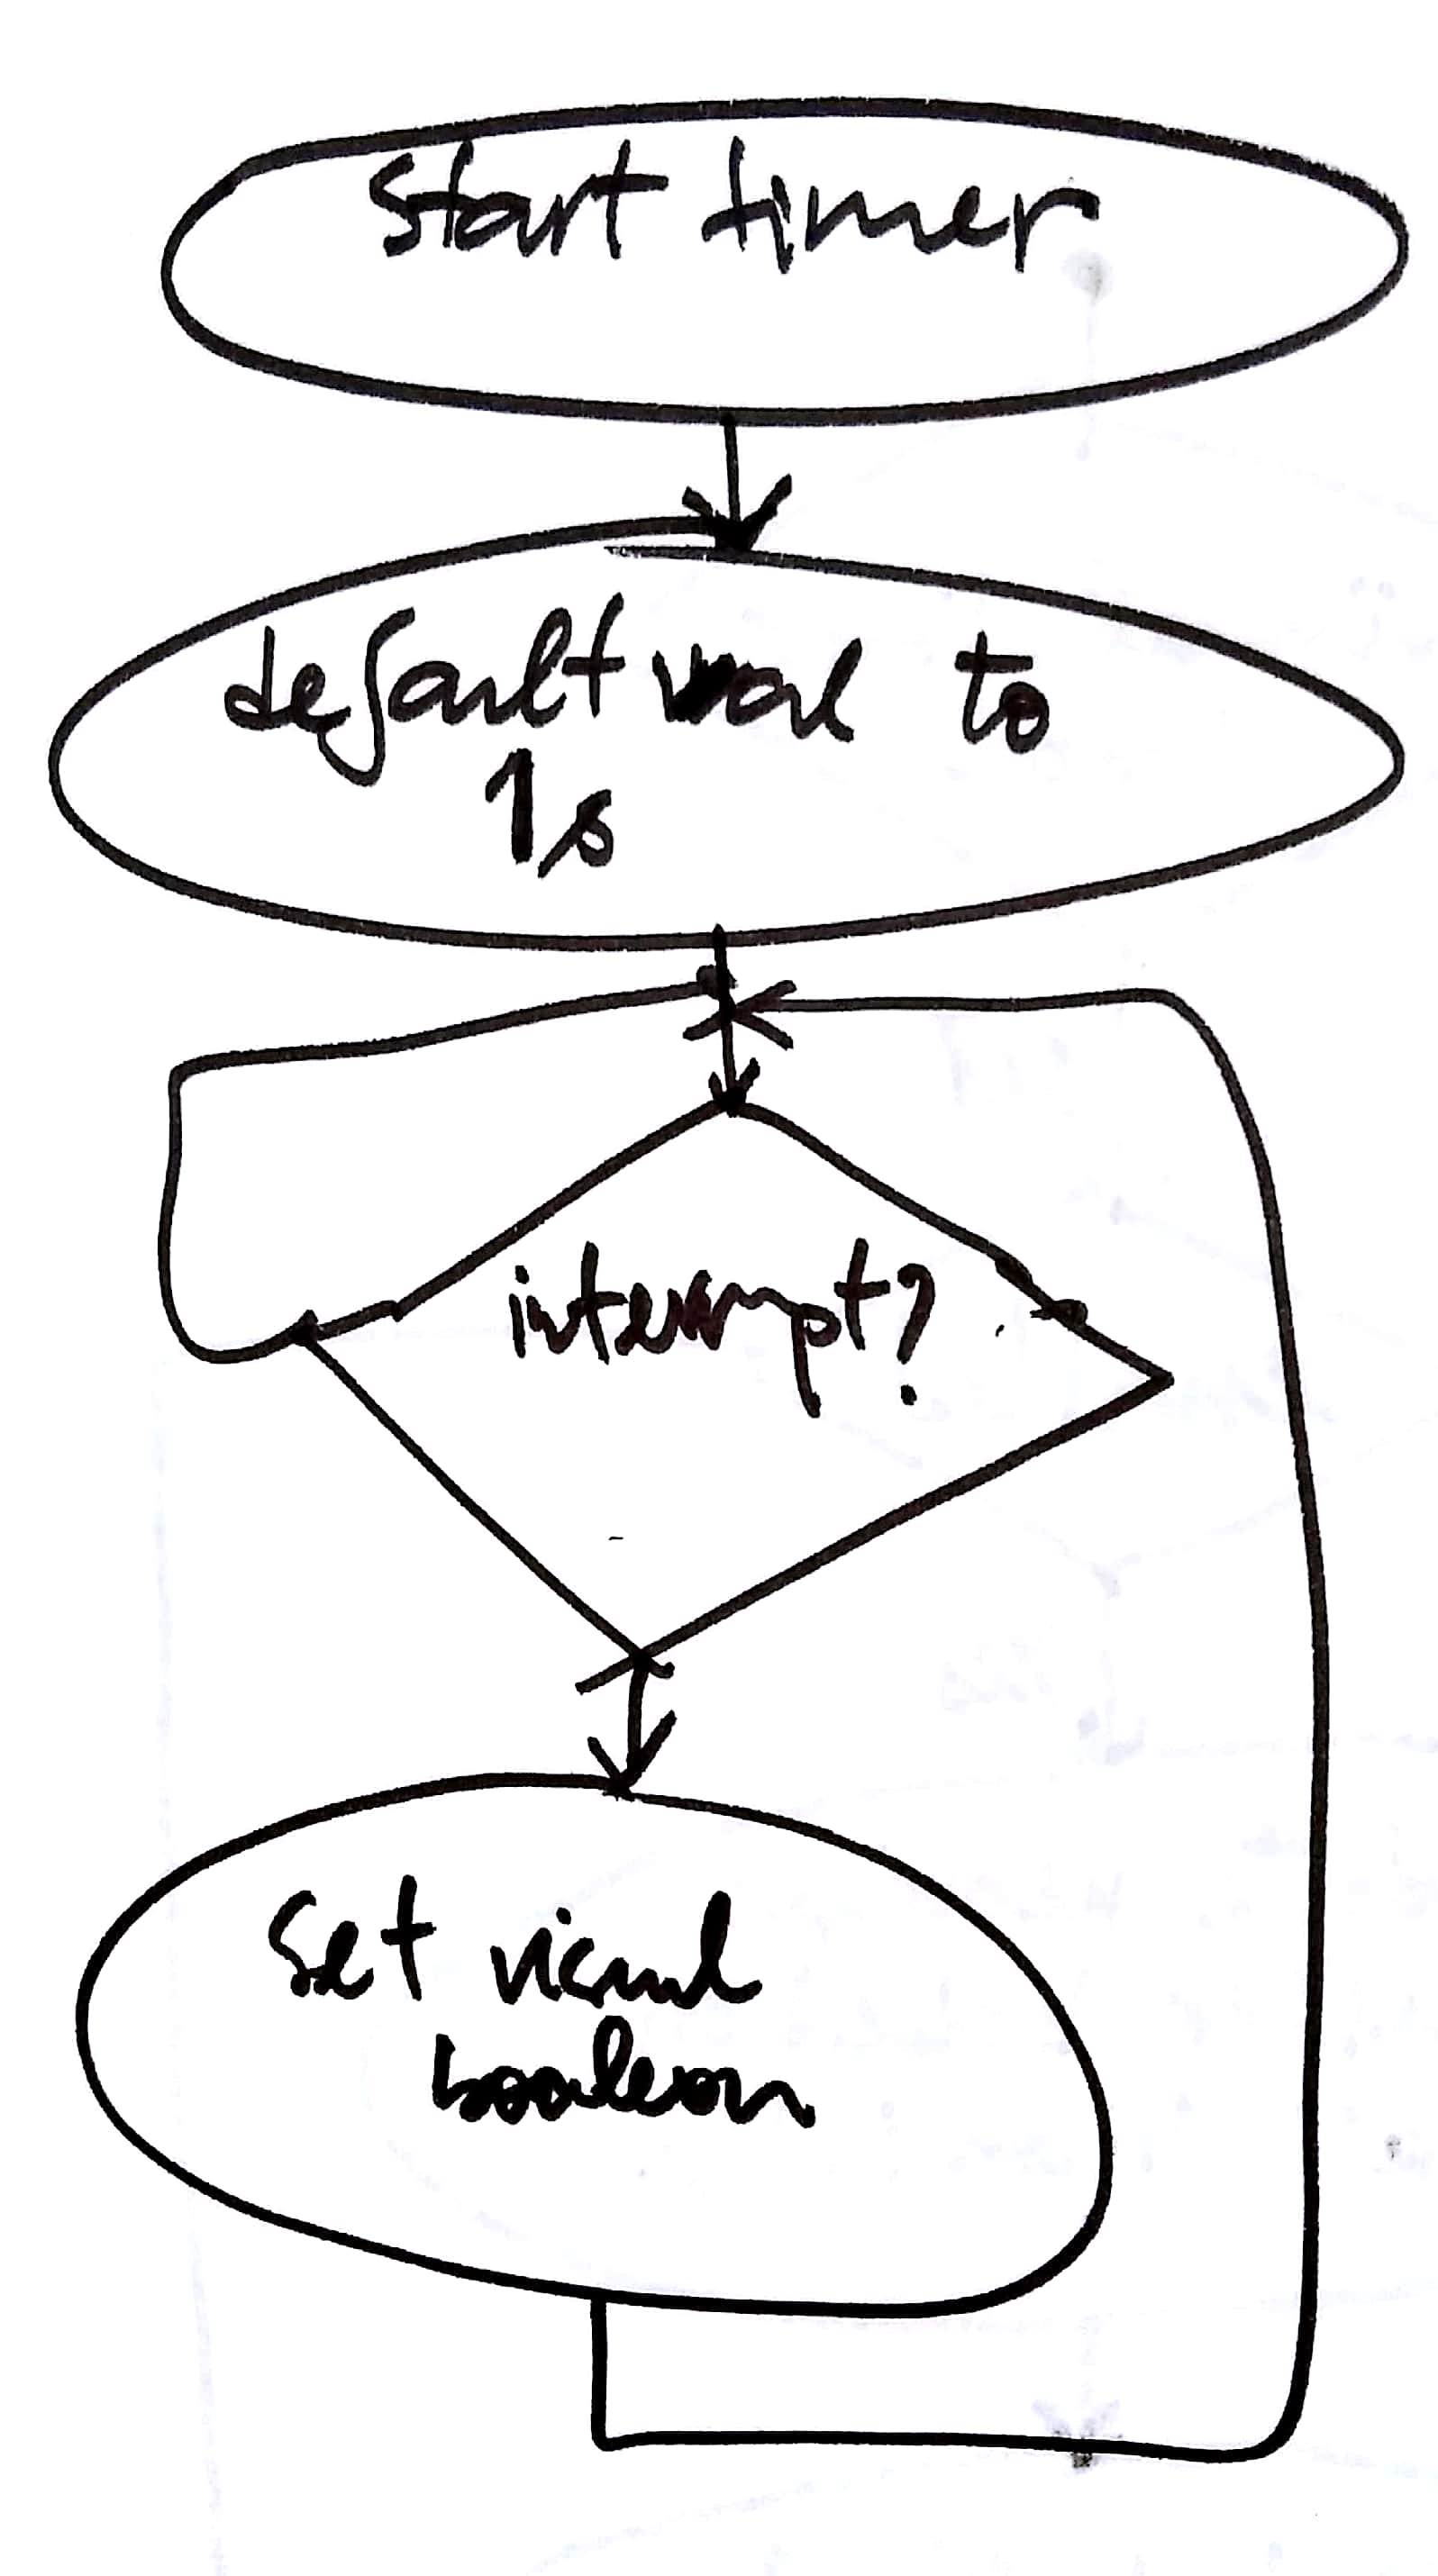
\includegraphics[scale=0.08]{timer_interrupt.jpg}
\caption{Flow diagram of the visual timer process.}
\label{fig:timer_interrupt}
\end{figure}
The \textit{visual update} process starts by verifying that the timer indicator of the specific visual module is set. If so, it then checks that the corresponding visual module is enabled. If the module is enabled, the neopixel buffer of the corresponding module is updated based on the pattern selected and an index indicating what should be the next iteration of the pattern. The process continues by display the pattern on the corresponding module and resetting the timer indicator.
\begin{figure}[ht]
\centering
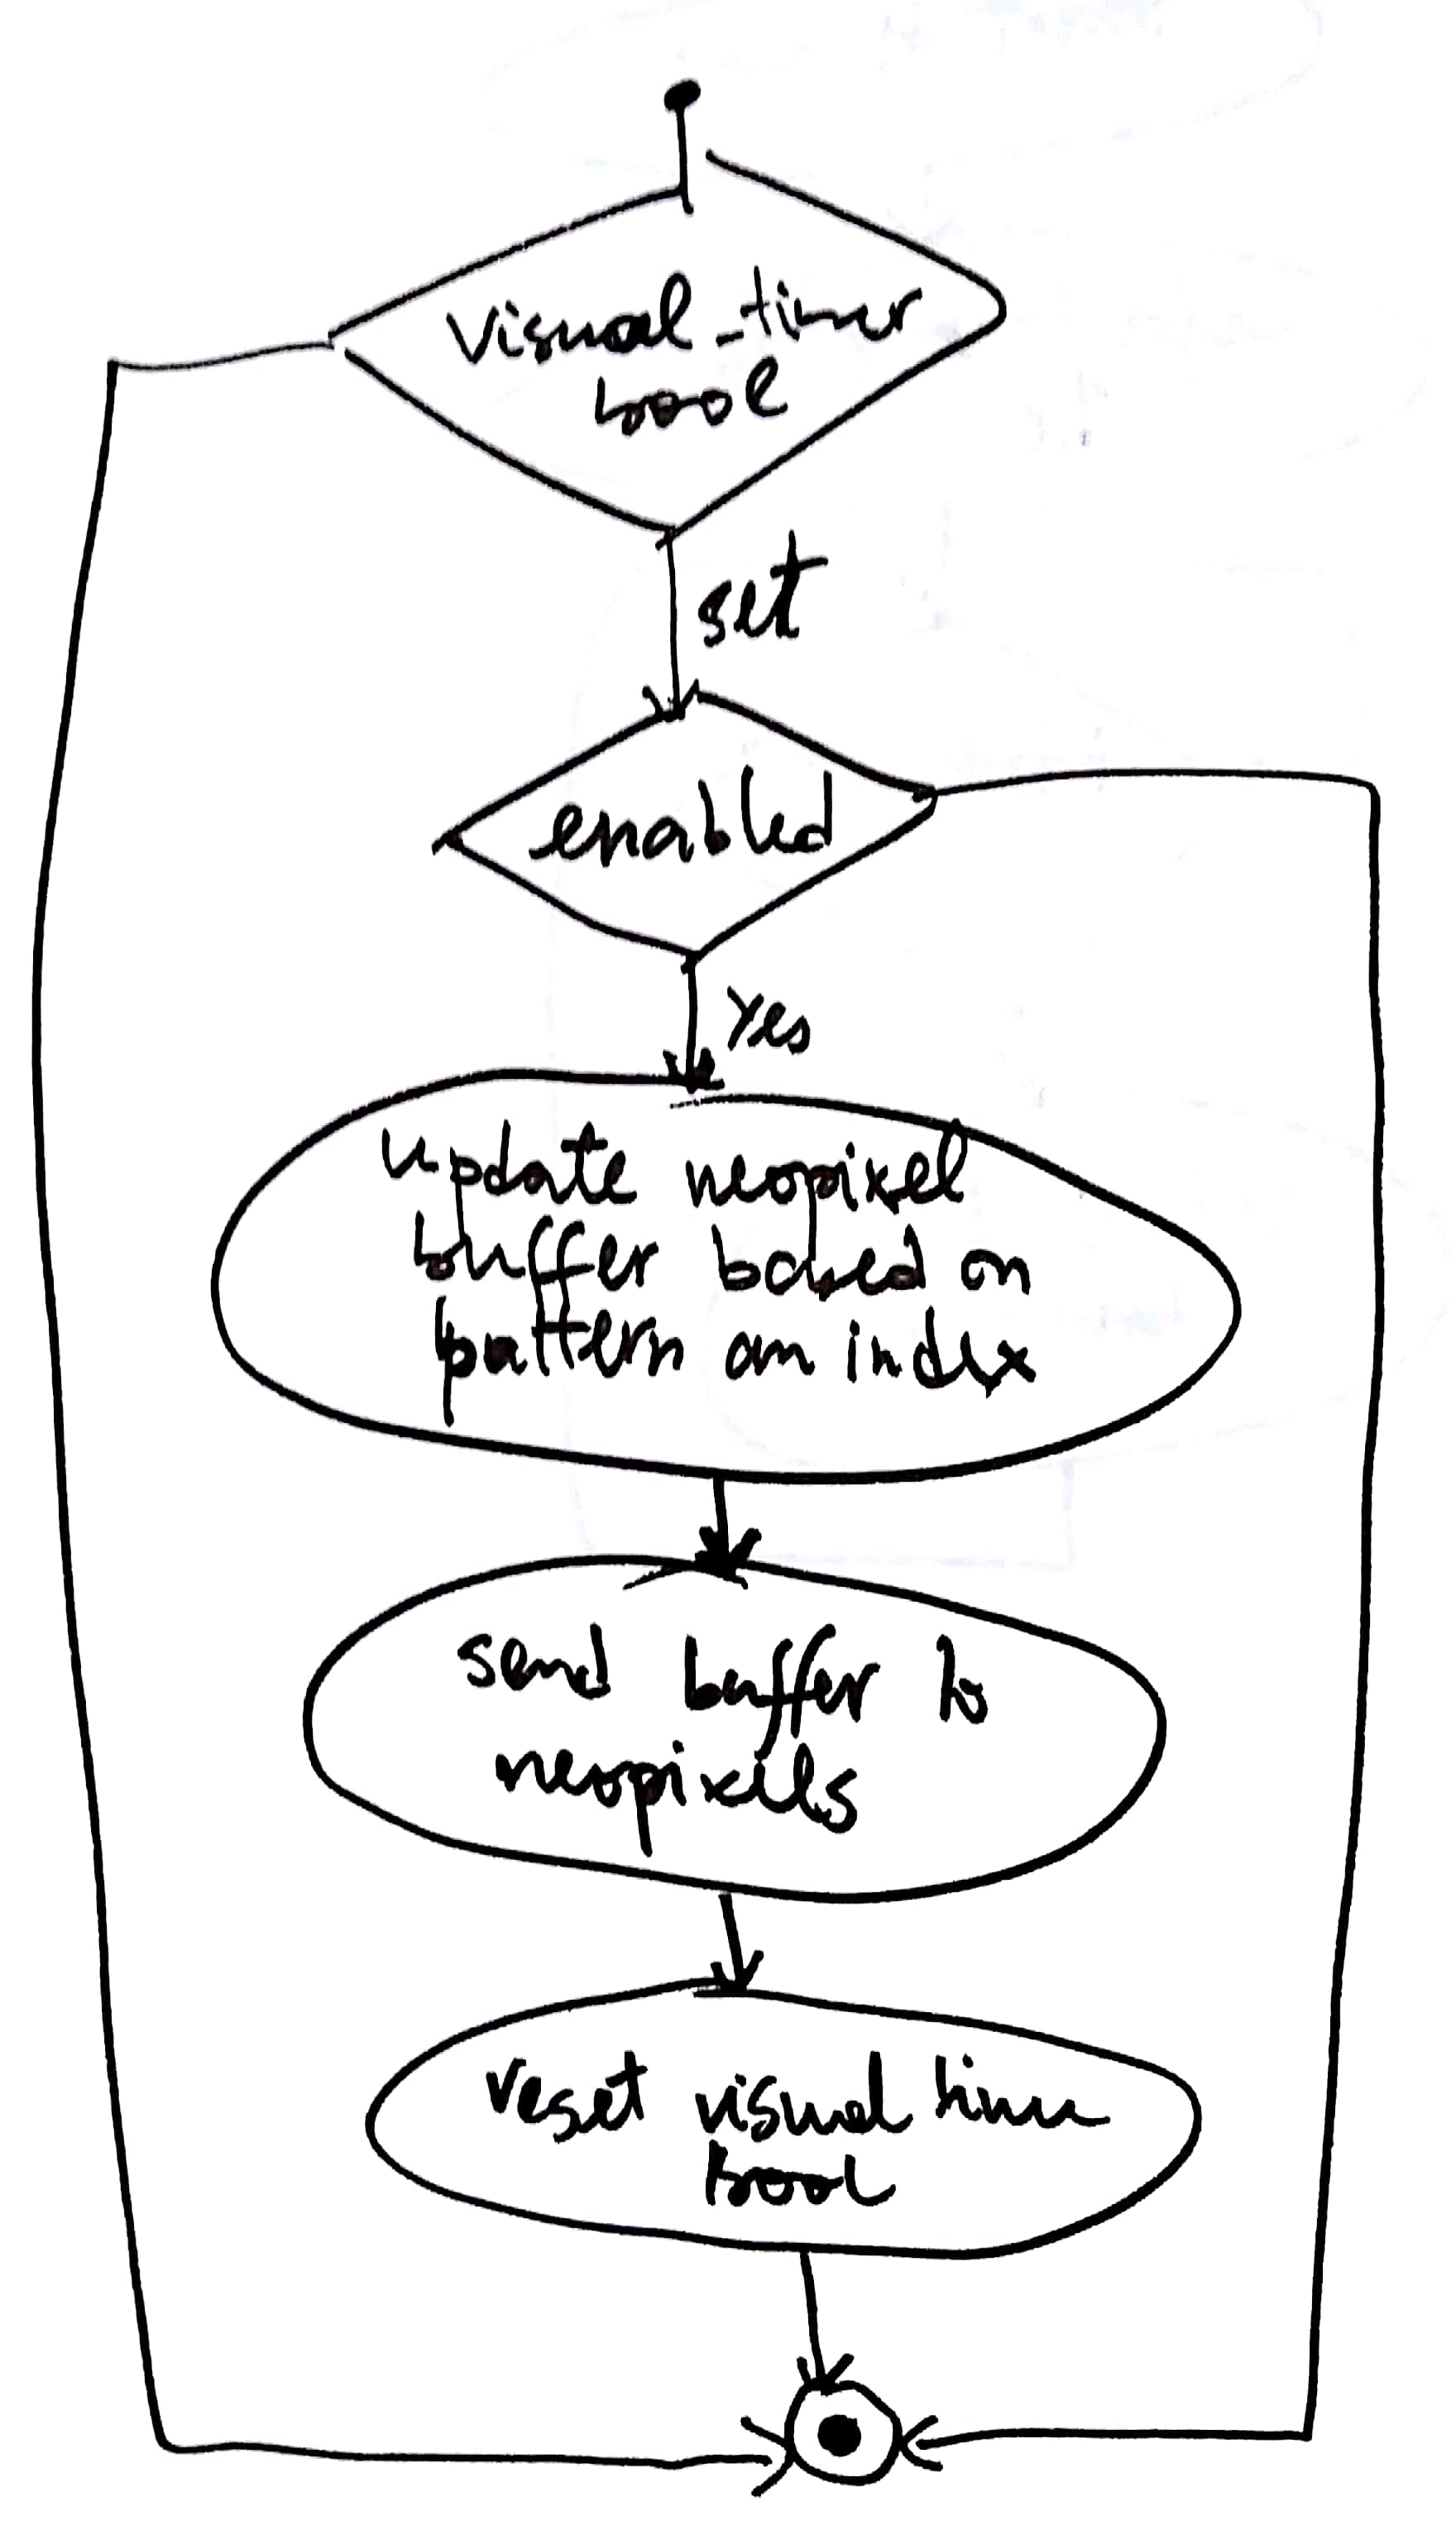
\includegraphics[scale=0.08]{visual_update.jpg}
\caption{Flow diagram of the visual update process. Each visual output module uses the same flow to update their visual.}
\label{fig:visual_update}
\end{figure}


\subsection{Alarm application}
This application has one main process. This process consists of calling another process (\textit{alarm\_update}) when the device is powered on or when an alarm has been updated in the EEPROM or has been triggered. \Cref{fig:alarm_update} gives the flow of this process. The \textit{alarm\_update} process loads the two alarms which will be triggered before the others, into Alarm A and B from the internal RTC. To make this decision, the alarms in the EEPROM are compared by converting the alarm into an integer value. The lower the value, the sooner the alarm will be triggered.
\begin{figure}[h!]
\centering
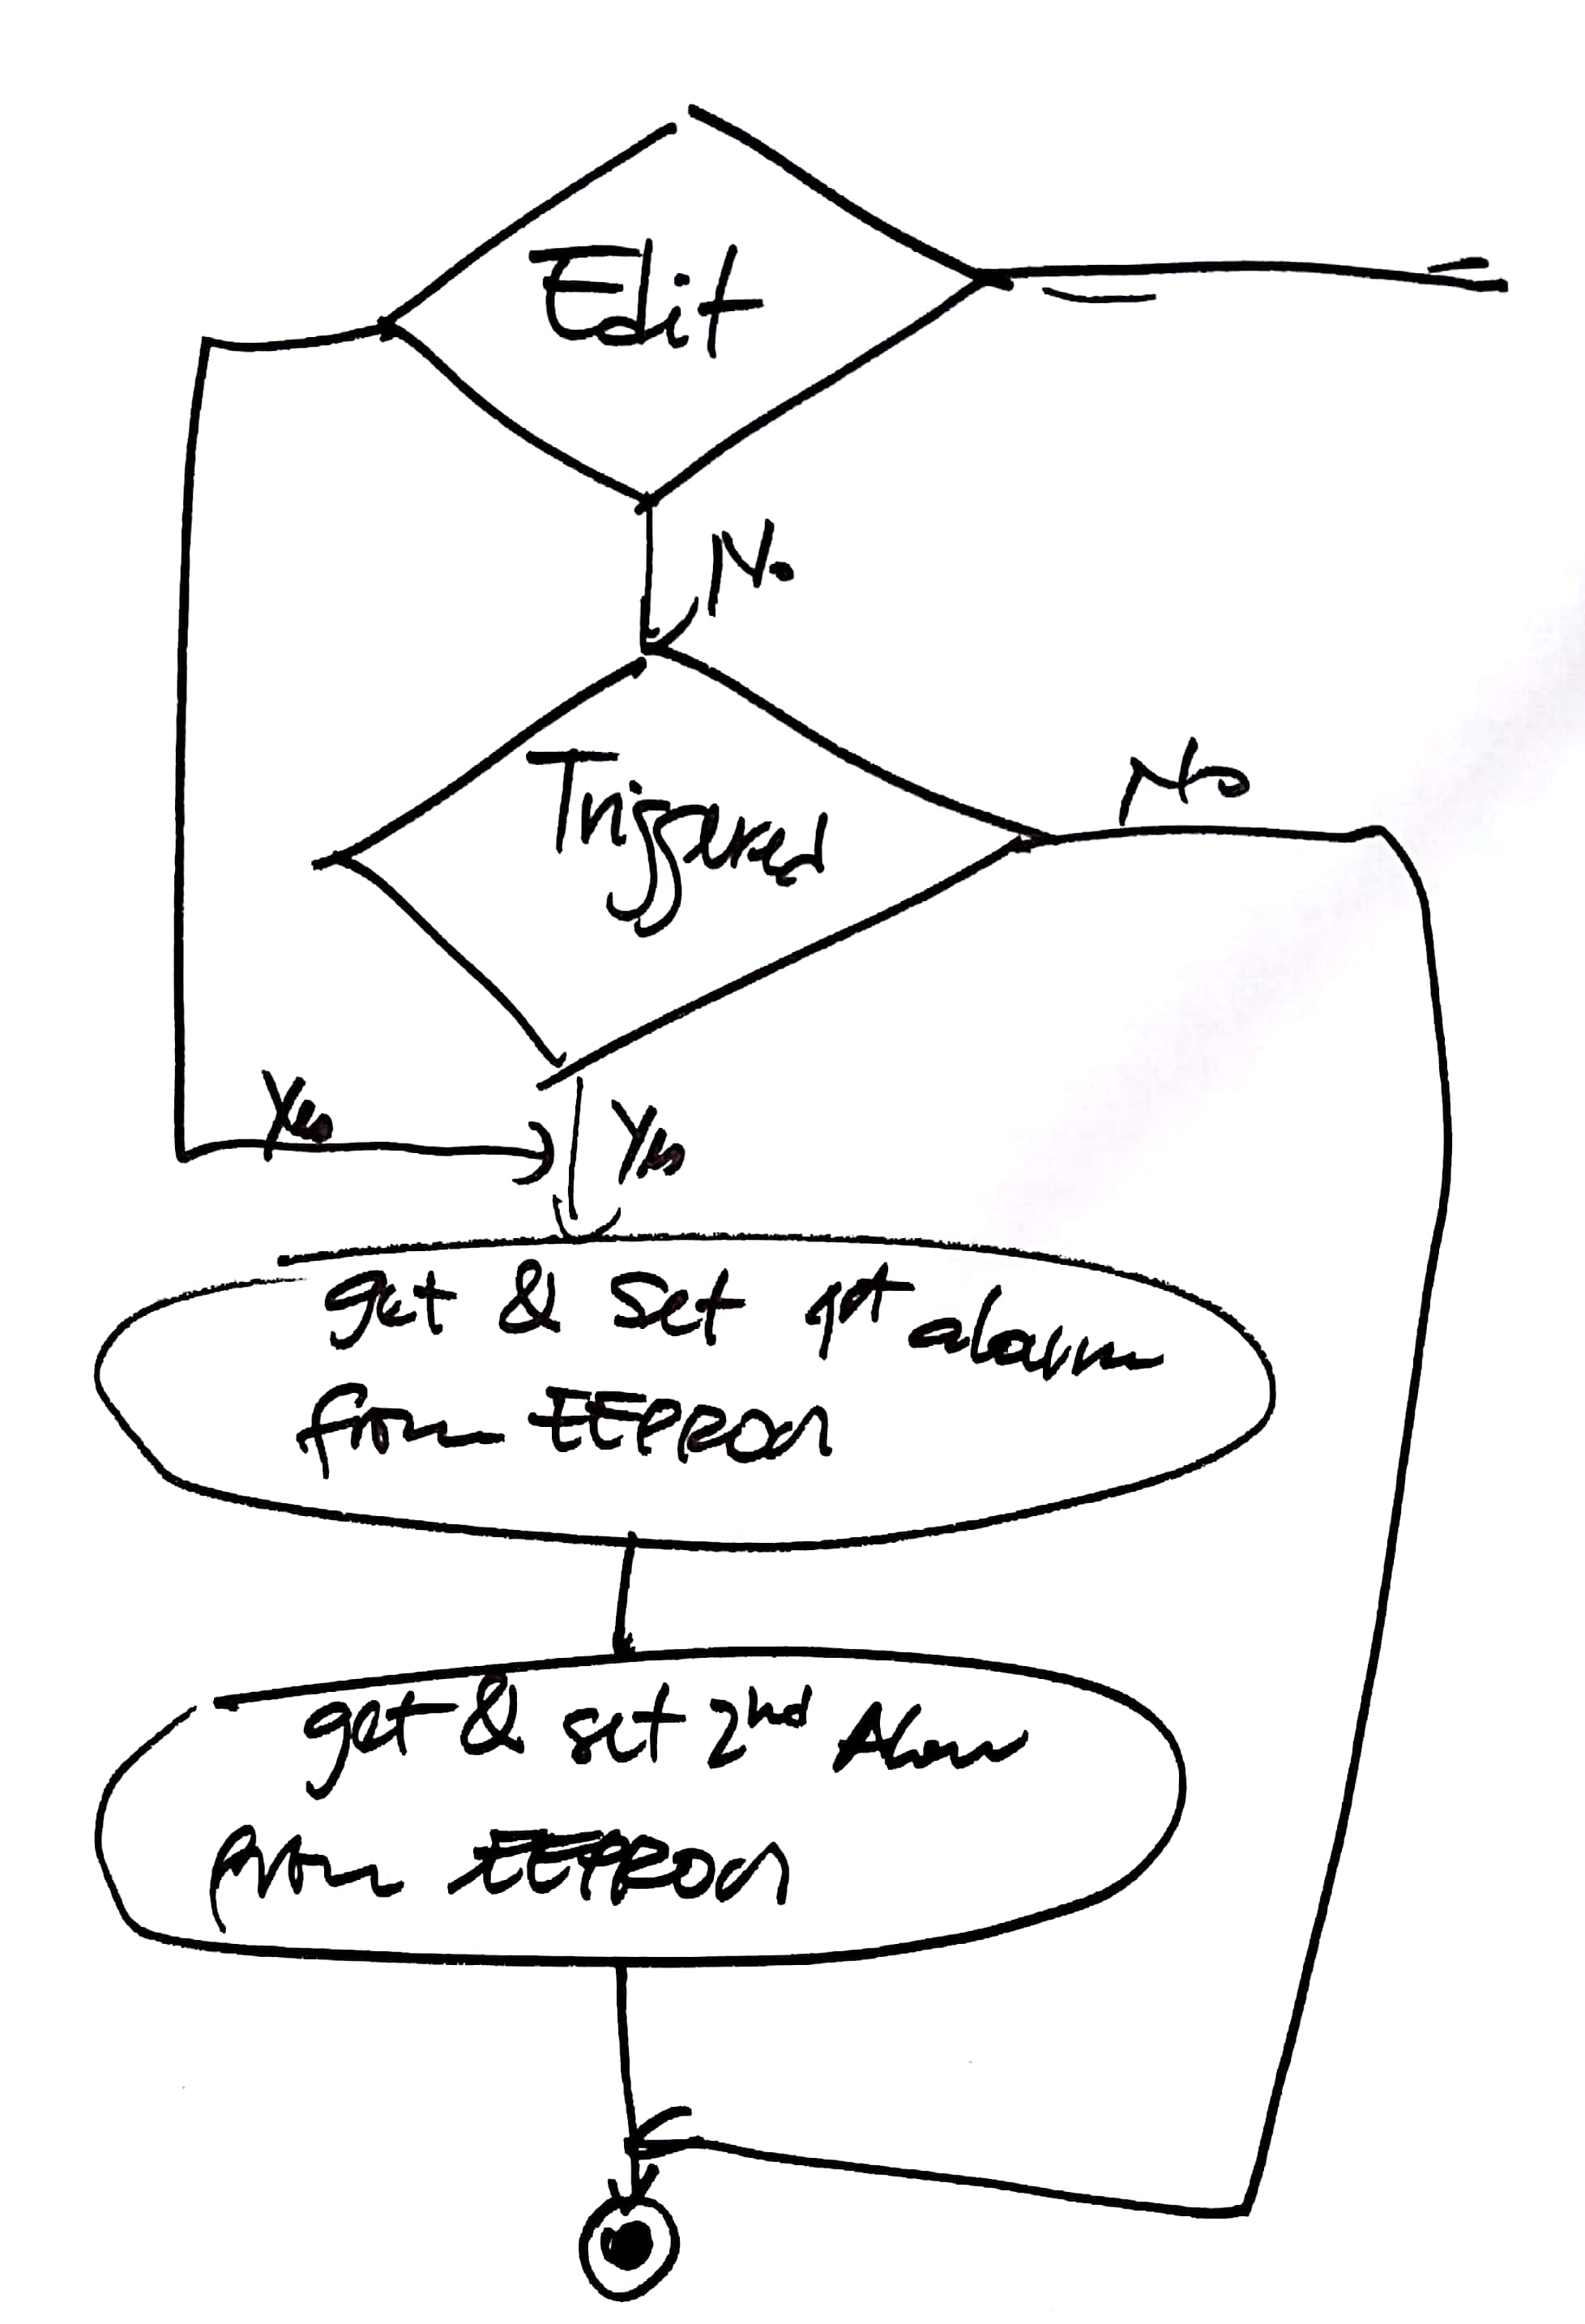
\includegraphics[scale=0.08]{alarm_update.jpg}
\caption{Flow diagram of the alarm update process.}
\label{fig:alarm_update}
\end{figure}


\subsection{Instruction application}
The operations performed in the instruction application can be divided into three principal operations, the \textit{DMA interrupt}, the \textit{device instruction update}, and the \textit{instruction fetch decode execute}.
\subsubsection{DMA interrupt}
There are two user input devices each using the DMA and a DMA buffer to store the byte sent to the STM. Each DMA generates an interrupt on data reception which is handled by the corresponding interrupt handler. When the device is powered on, the CPU initialise the communication with the input device, then it continuously observes the DMA and generates an interrupt when data is received. When this occurs, the DMA interrupt handler then set a boolean value to indicate that data was received from the input device. The flow of the process described above is illustrated in \cref{fig:dma_interrupt}. 
\begin{figure}[ht]
\centering
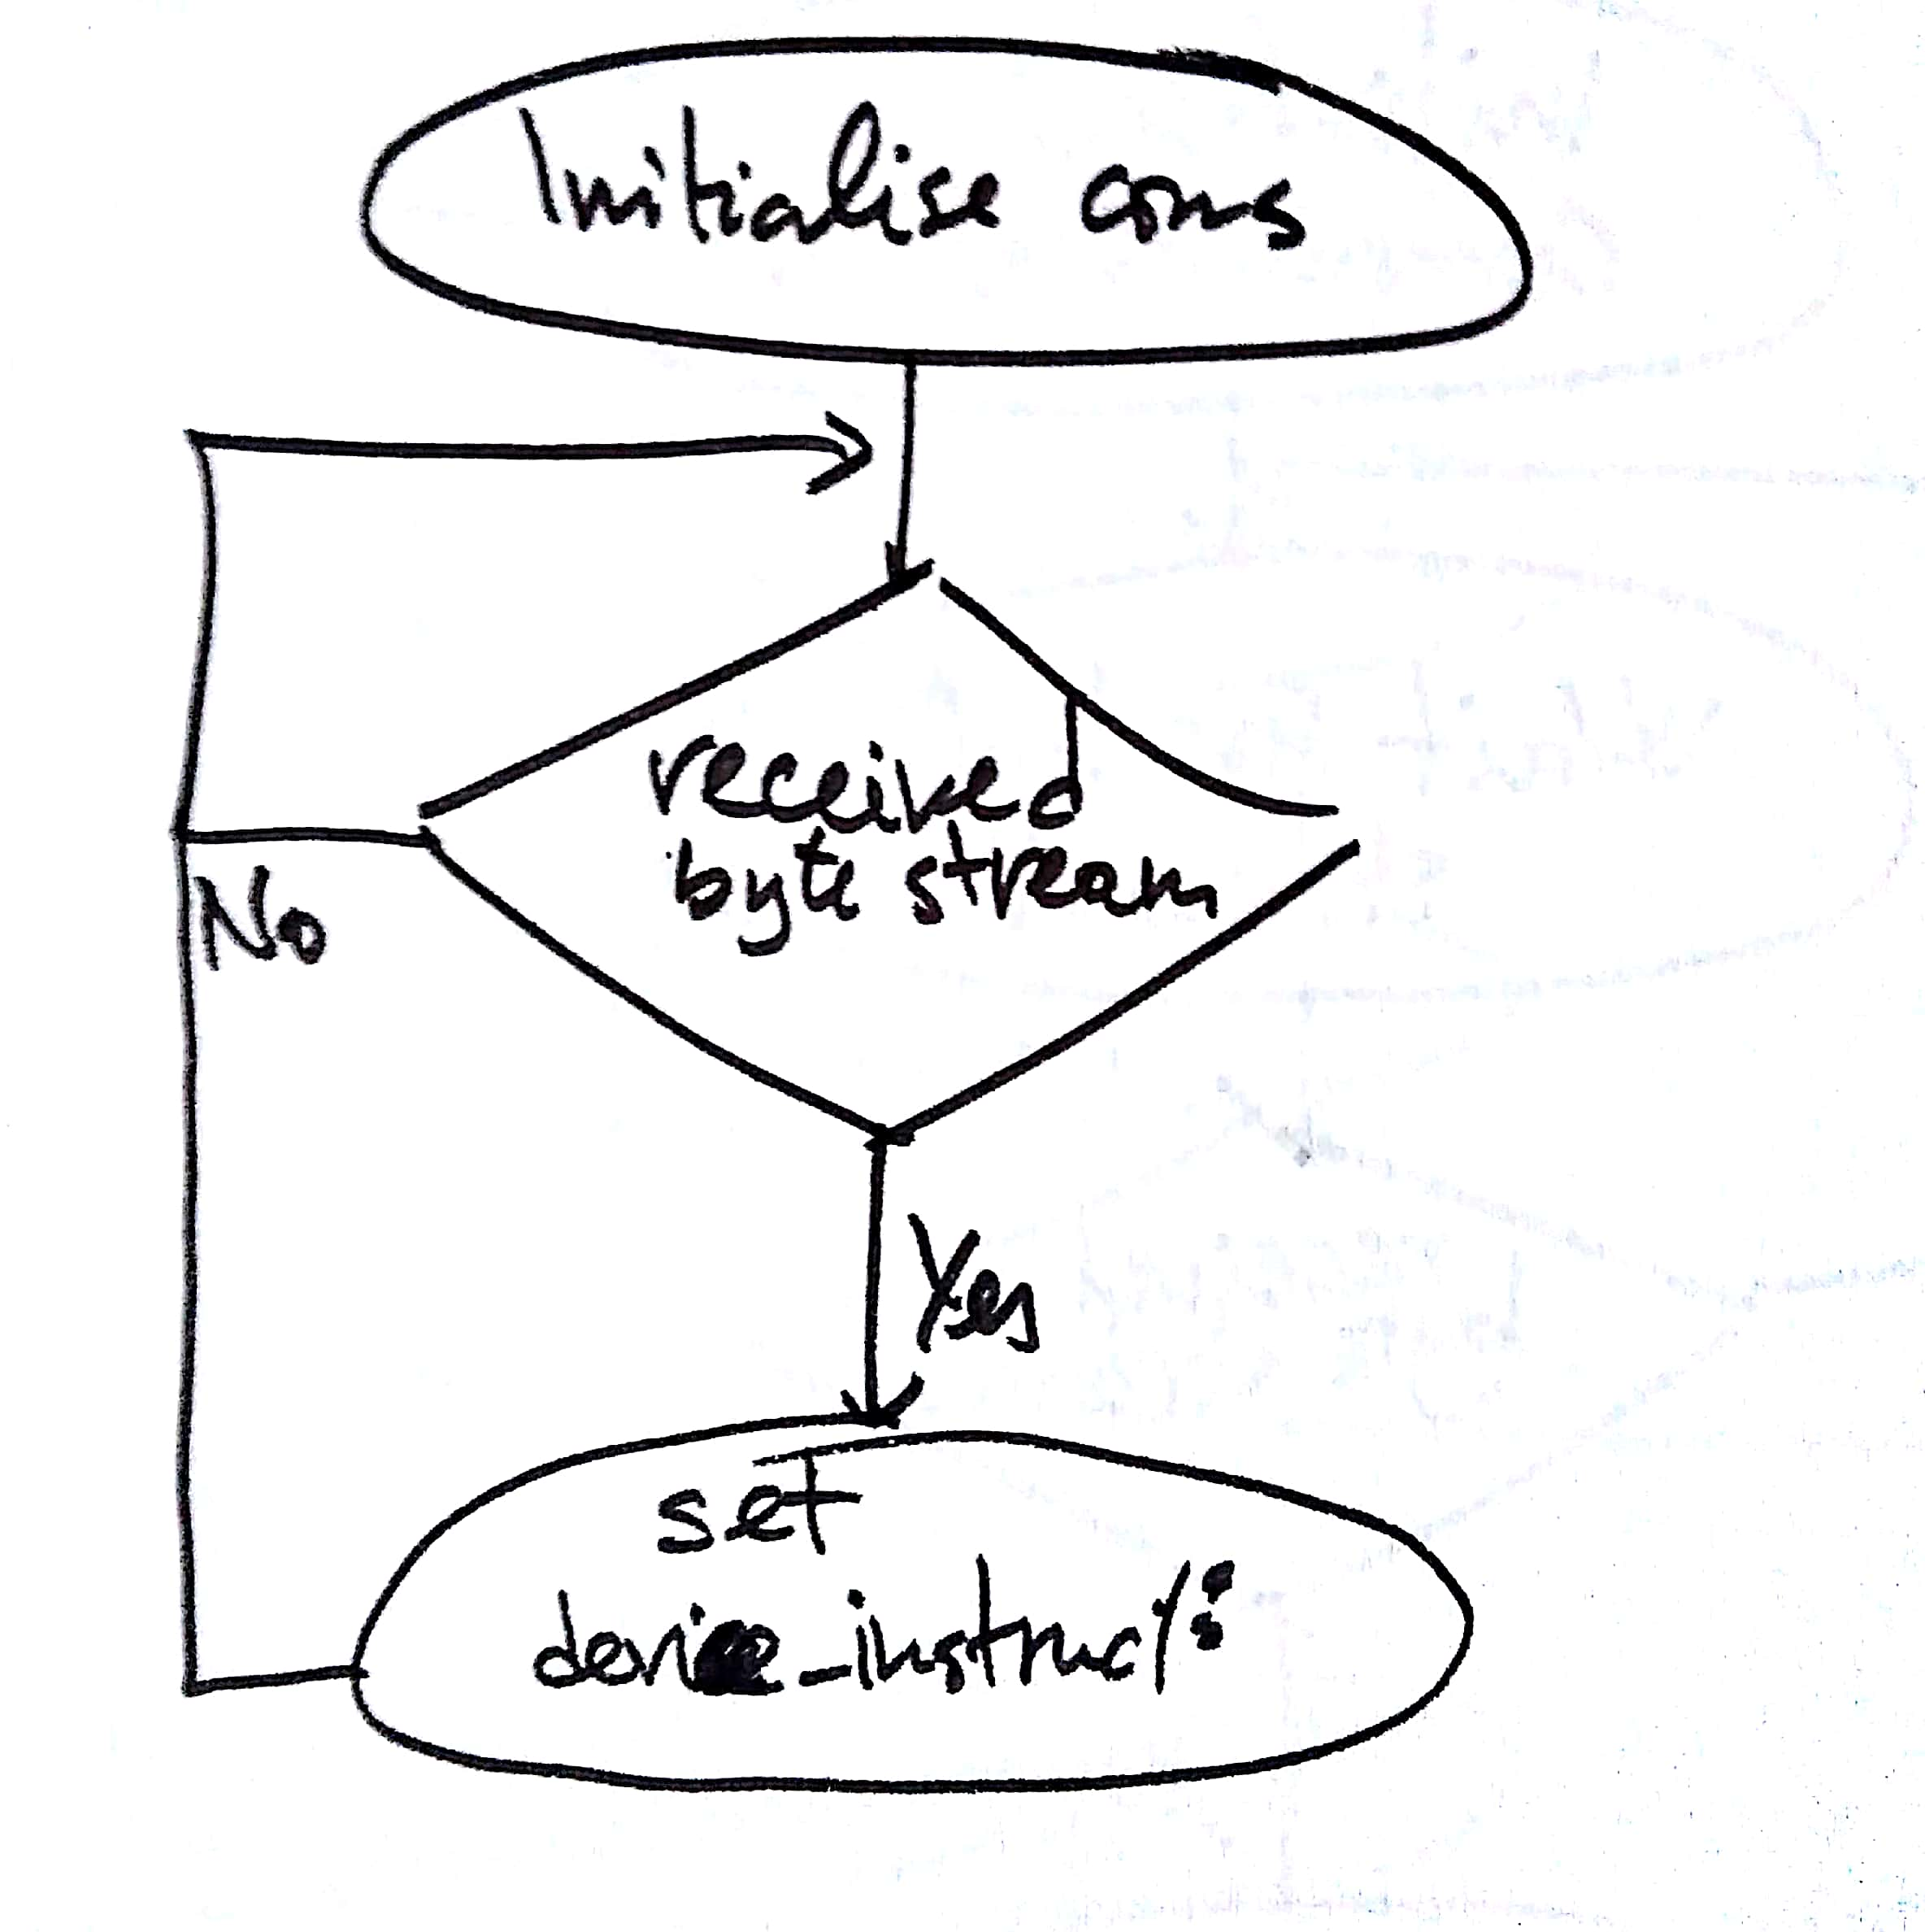
\includegraphics[scale=0.08]{dma_interrupt.jpg}
\caption{Flow diagram of the DMA process.}
\label{fig:dma_interrupt}
\end{figure}

\subsubsection{Device instruction update}
The purpose of this process is to convert the data stored in the DMA Buffer into instructions and add these instructions to the instruction buffer. When the process is called, the boolean set by the DMA interrupt process is evaluated. When its value is \textit{reset}, it implies that the DMA buffer did not receive any new instructions. If the boolean was set, the DMA buffer is divided into sections of eight bytes each (size of an instruction) and each section is converted into instructions, then added to the instruction queue and the boolean is reset. Prior the conversion of the DMA buffer section to instructions, the data contained in these sections are analysed and sections which do not match any instruction type are discarded. The flow of this process is illustrated in \cref{fig:device_instructionUpdate}. 
\begin{figure}[ht]
\centering
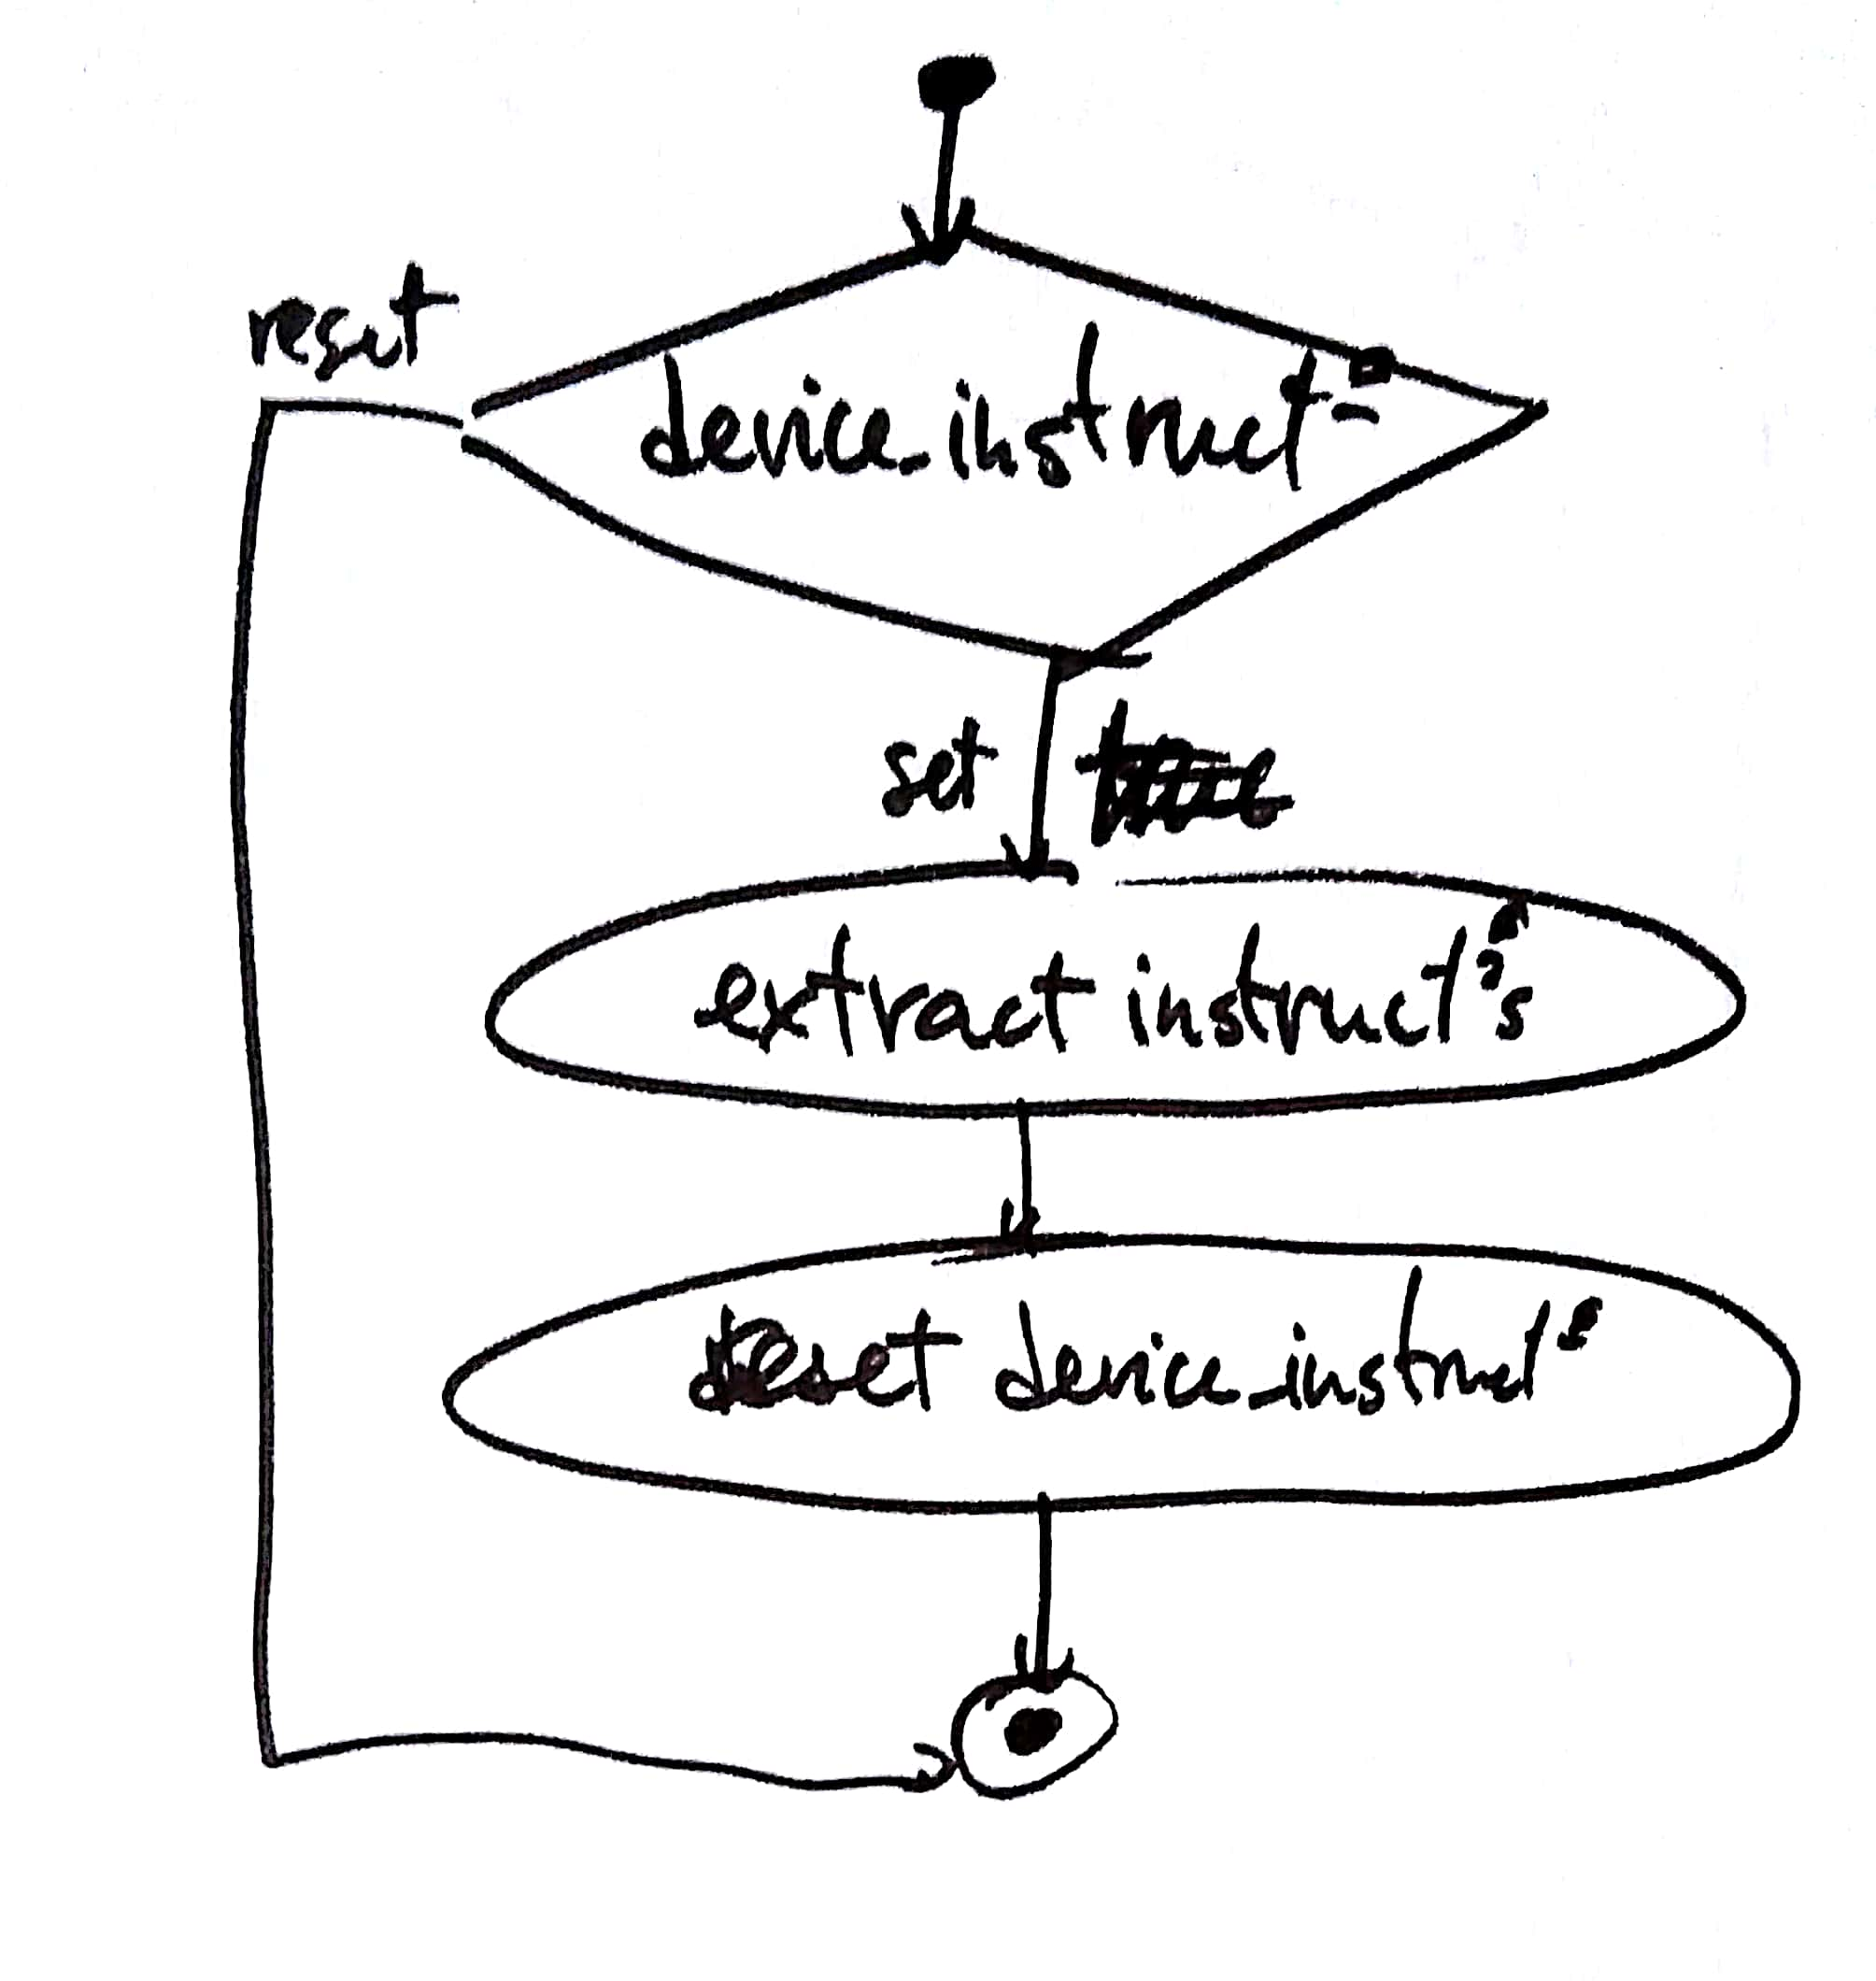
\includegraphics[scale=0.08]{device_instructionUpdate.jpg}
\caption{Flow diagram of the input device instruction update. Both Nextion screen and Bluetooth application uses the same flow to update the instruction queue.}
\label{fig:device_instructionUpdate}
\end{figure}

\subsubsection{Instruction Fectch Decode Execute (IFDE)}\label{IFDE}
The IFDE's purpose is to fetch, decode and execute the instructions in the instruction queue. This process starts by checking that there are instructions in the instruction queue. It then fetches these instructions one by one, decode and execute the instructions. The process stops when the instruction queue is empty. This process is illustrated in \cref{fig:ifde} and a portion of the code used for its implementation is shown in listing \ref{code:ifde}. .
\begin{figure}[ht]
\centering
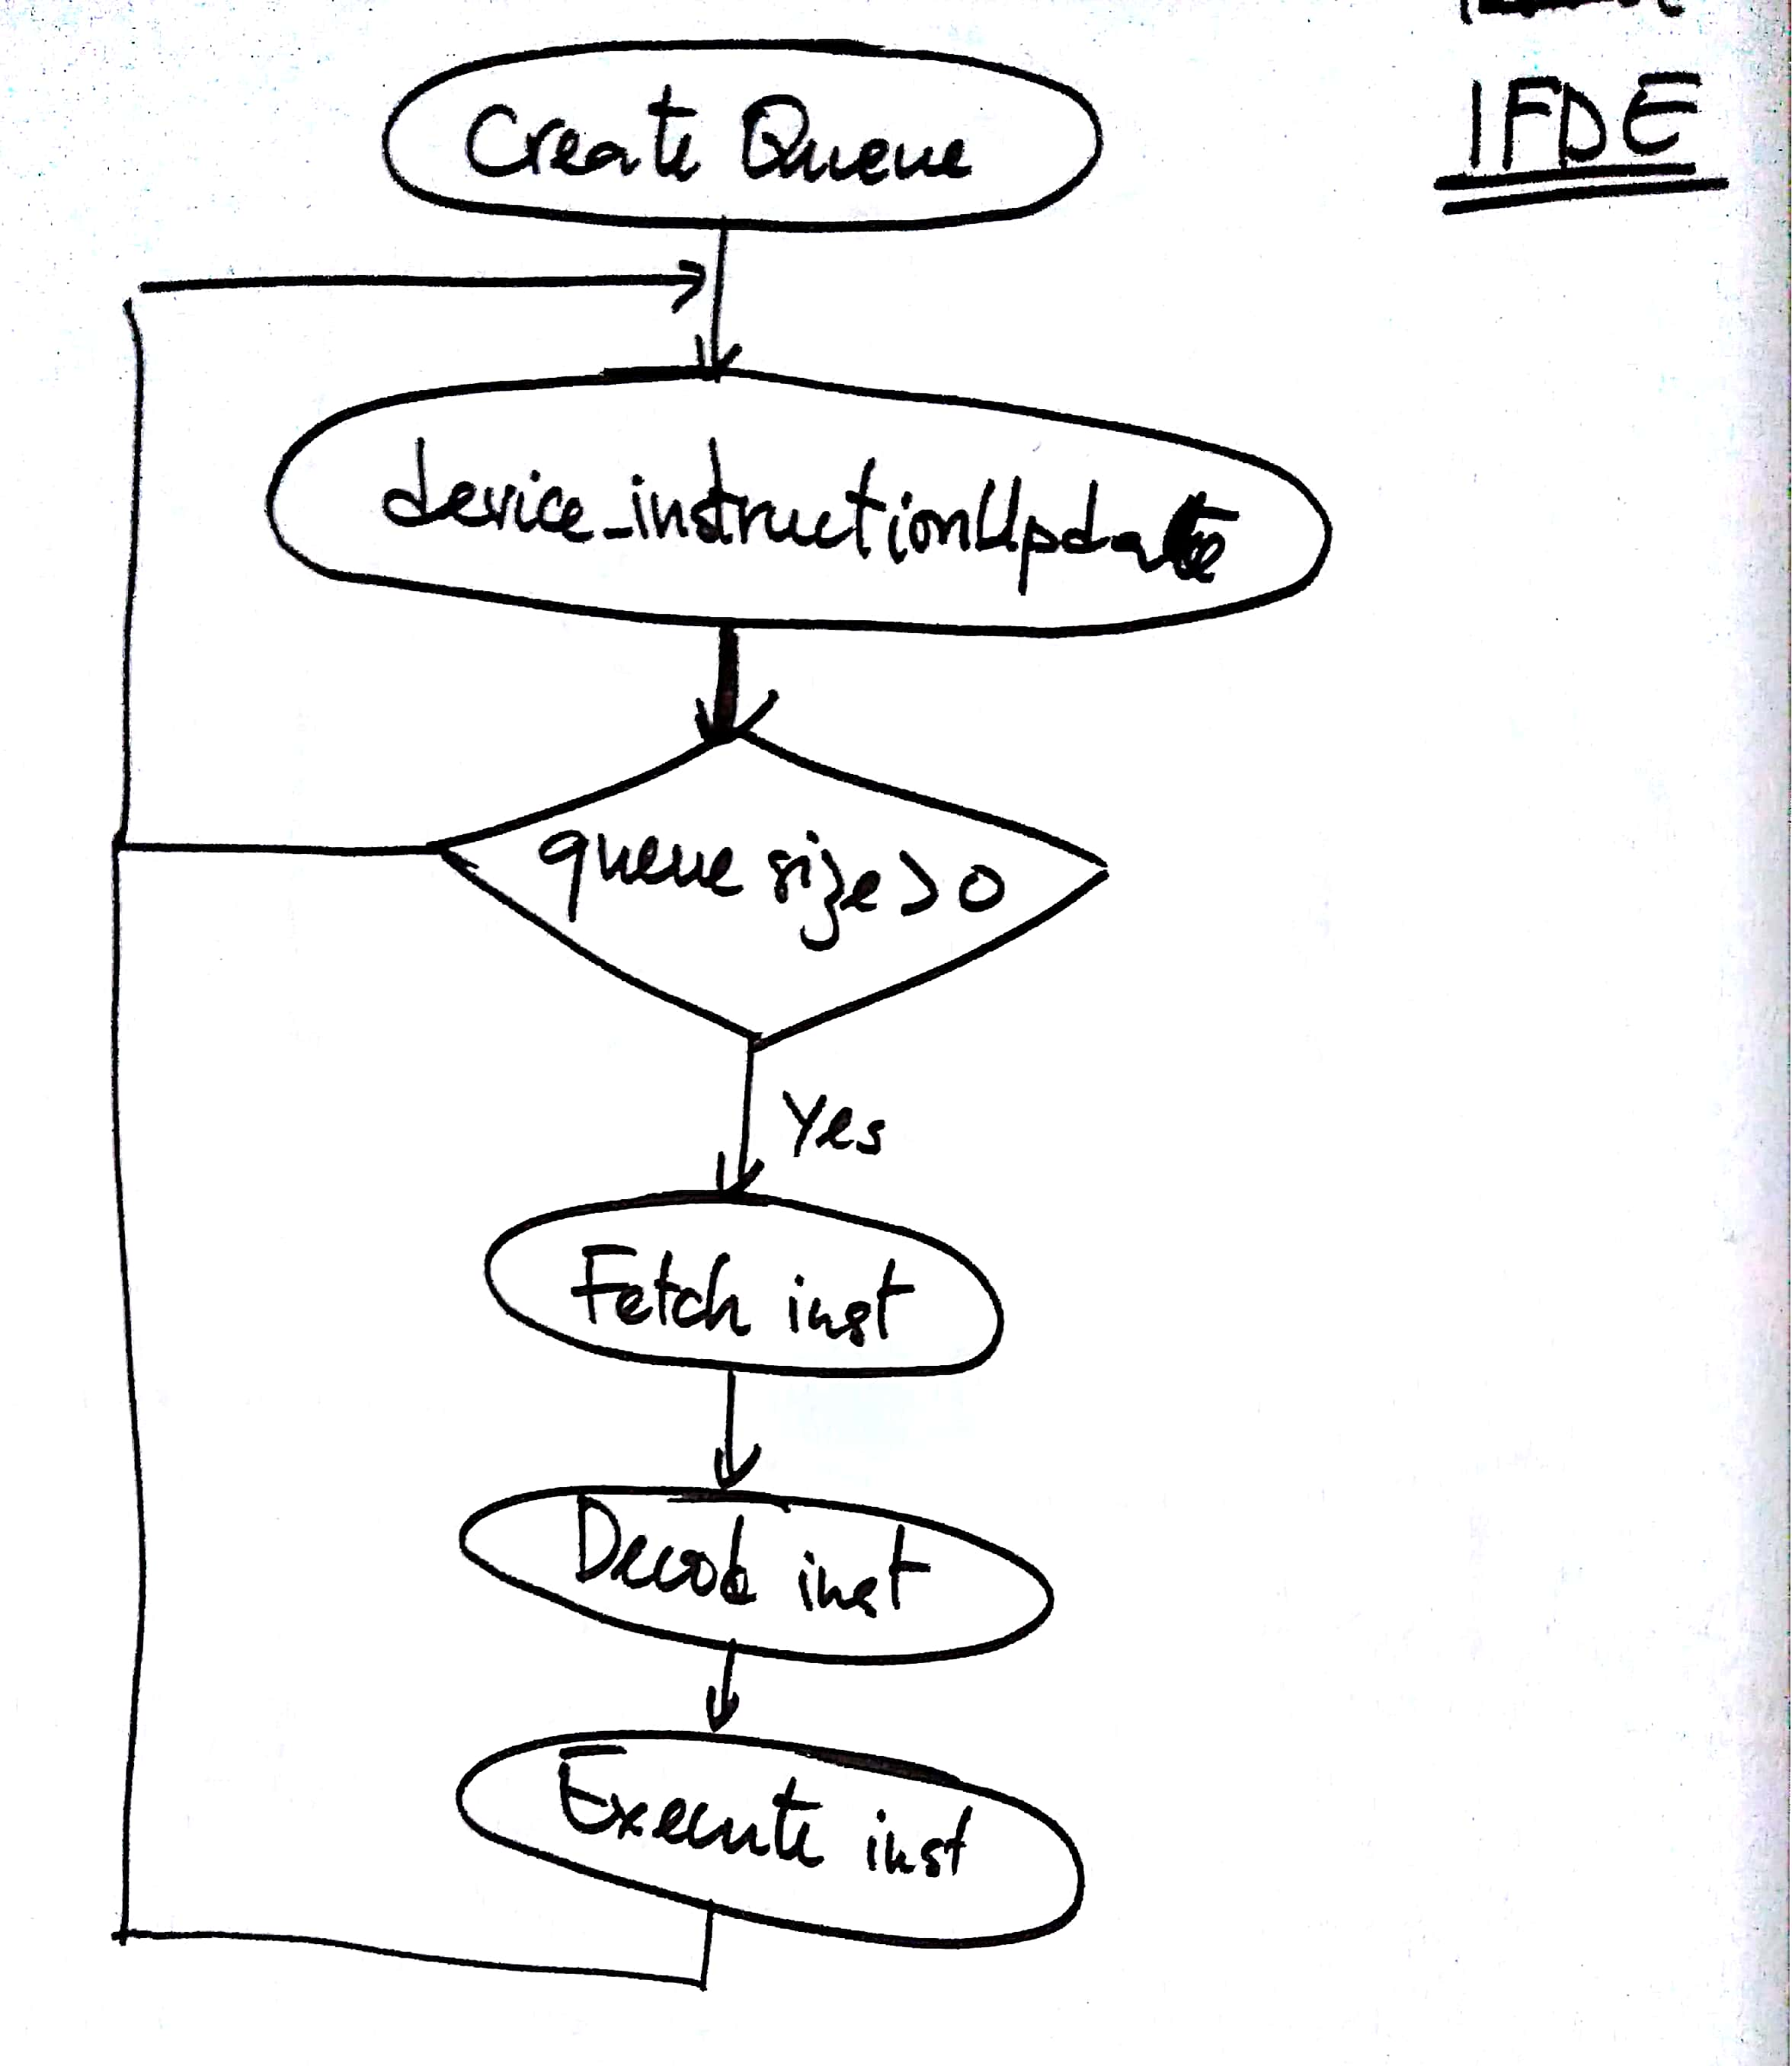
\includegraphics[scale=0.09]{ifde.jpg}
\caption{Flow diagram of the IFDE process.}
\label{fig:ifde}
\end{figure}
\begin{lstlisting}[language=C, caption=Instruction Fetch Decode Execute, label=code:ifde]
/**
 * @brief    Execute instructions from instruction queue
 */
void instruction_execute(void){
    RTC_ClockTypeDef clock;
    AlarmTypeDef alarm;
    // check if the queue is empty
    while(InstructionQueue_isEmpty(instruction_queue)){
        // Fecth instruction
        InstructionTypeDef _instruction = InstructionQueue_dequeue(instruction_queue);
        // Decode and Execute instruction
        switch(_instruction.instrution[0]){
        /* External RTC instructions */
        case 0x01:
            // set clock
            clock.date.RTC_Year=_instruction.instrution[1];
            clock.date.RTC_Month=_instruction.instrution[2];
            ...
            rtc_setClockStruct(&clock);
            break;
        case 0x02:
            // get clock
            instruction_nextionStart();
            ...            
            instruction_nextionSendStr("home.t2.txt=", rtc_monthToString(clock.date.RTC_Month) );
            instruction_nextionSendInt("home.n4.val=",2000+clock.date.RTC_Year);
            instruction_nextionStop();
              break;        
        ...
        }
    }
}
\end{lstlisting}
After the instruction \textit{\_instruction} is extracted from the \textit{instruction\_queue}, the first byte (\textit{\_instruction[0]}) is used to decode the instruction based on the instruction set defined in \cref{table:instruction_set}. There are two types of instructions, the \textit{get instructions} and the \textit{set instructions}. The \textit{set instructions} contains parameters used to update the hardware modules of the NPSC. The \textit{get instructions} are used to signal the NPSC that the input device required some parameters update. Each device response to the \textit{get instructions} is different. The Bluetooth response is not complex and consists on sending an instruction (eight bytes) to the Bluetooth device. The Nextion touchscreen response is more complicated; after sending a \textit{get instruction} to the STM, the Nextion touchscreen waits for instruction. The STM replies to this request by starting a three phases protocol consisting of:
\begin{itemize}
\item \textbf{instruction\_nextionStart()}: The STM sends random data to signal the touchscreen that useful data will arrive.
\item \textbf{instruction\_nextionSend$<$type$>$(char *, type)}: Special Nextion commands are used to update the screen parameters.
\item \textbf{instruction\_nextionStop()}: The STM ends the transmission by sending a \textit{"com stop"} instruction to the screen. 
\end{itemize}

%%%%%%%%%%%%%%%%%%%%%%%%%%%%%%%%%%%%%%%%%%%%%%%%%%%%%%%%%%%%%%%%%%%%%%%%%%%%%%%%%%%%
% SECTION: Main
%%%%%%%%%%%%%%%%%%%%%%%%%%%%%%%%%%%%%%%%%%%%%%%%%%%%%%%%%%%%%%%%%%%%%%%%%%%%%%%%%%%%
\section{Main}
The main or the master application has one unique role: \textit{to start all processes}. This application calls the initialization functions of each level which start the hardware communication protocols, the instruction update process, the IFDE process and so forth. 

%%%%%%%%%%%%%%%%%%%%%%%%%%%%%%%%%%%%%%%%%%%%%%%%%%%%%%%%%%%%%%%%%%%%%%%%%%%%%%%%%%%%
% SECTION: Utilities
%%%%%%%%%%%%%%%%%%%%%%%%%%%%%%%%%%%%%%%%%%%%%%%%%%%%%%%%%%%%%%%%%%%%%%%%%%%%%%%%%%%%
\section{Utilities}
This module contains all functions used by other modules. \Cref{table:utilities} describes the use of each file in the Utilities module.
\begin{table}[h!]
	\centering
	\caption{Description of the files at the Utilities level.}
	\label{table:utilities}
	\begin{tabular}{cp{30em}}
		\hline
		\hline
		\toprule
		\textbf{File Name} & \textbf{Description}\\
		\bottomrule
		\toprule
		queue & Contains functions to create a queue of a certain data type, add and remove elements from the queue. \\
		\midrule
		utils & Contains functions, variables and type definitions used other software modules at different levels of the hierarchy.\\
		\bottomrule
		\hline
		\hline
	\end{tabular}
\end{table}